%%%%%%%%%%%%%%%%%%%%%%%%%%%%%%%%%%%%%%%%%
% Journal Article
% LaTeX Template
% Version 1.4 (15/5/16)
%
% This template has been downloaded from:
% http://www.LaTeXTemplates.com
%
% Original author:
% Frits Wenneker (http://www.howtotex.com) with extensive modifications by
% Vel (vel@LaTeXTemplates.com)
%
% License:
% CC BY-NC-SA 3.0 (http://creativecommons.org/licenses/by-nc-sa/3.0/)
%
%%%%%%%%%%%%%%%%%%%%%%%%%%%%%%%%%%%%%%%%%

%----------------------------------------------------------------------------------------
%	PACKAGES AND OTHER DOCUMENT CONFIGURATIONS
%----------------------------------------------------------------------------------------

%\documentclass[10pt]{article} % Single column

\documentclass[colorinlistoftodos,twoside,twocolumn,10pt]{article} % Two column

\usepackage{blindtext} % Package to generate dummy text throughout this template 

\usepackage[sc]{mathpazo} % Use the Palatino font
\usepackage[T1]{fontenc} % Use 8-bit encoding that has 256 glyphs
\linespread{1.05} % Line spacing - Palatino needs more space between lines
\usepackage{microtype} % Slightly tweak font spacing for aesthetics

\usepackage[spanish]{babel} % Language hyphenation and typographical rules

\usepackage[hmarginratio=1:1,top=20mm,columnsep=15mm, left=12mm, right=12mm, bottom=25mm]{geometry} % Document margins
\usepackage[hang, small,labelfont=bf,up,textfont=it,up]{caption} % Custom captions under/above floats in tables or figures
\usepackage{booktabs} % Horizontal rules in tables

\usepackage{lettrine} % The lettrine is the first enlarged letter at the beginning of the text

\usepackage{enumitem} % Customized lists
\setlist[itemize]{noitemsep} % Make itemize lists more compact

\usepackage{abstract} % Allows abstract customization
\renewcommand{\abstractnamefont}{\normalfont\bfseries} % Set the "Abstract" text to bold
\renewcommand{\abstracttextfont}{\normalfont\small\itshape} % Set the abstract itself to small italic text

\usepackage{titlesec} % Allows customization of titles
\renewcommand\thesection{\Roman{section}} % Roman numerals for the sections
\renewcommand\thesubsection{\roman{subsection}} % roman numerals for subsections
\titleformat{\section}[block]{\large\scshape\centering}{\thesection.}{1em}{} % Change the look of the section titles
\titleformat{\subsection}[block]{\large}{\thesubsection.}{1em}{} % Change the look of the section titles

\usepackage{fancyhdr} % Headers and footers
\pagestyle{fancy} % All pages have headers and footers
\fancyhead{} % Blank out the default header
\fancyfoot{} % Blank out the default footer
\fancyhead[C]{Music Genre Classifier} % Custom header text
\fancyfoot[RO,LE]{\thepage} % Custom footer text

\usepackage{titling} % Customizing the title section

\usepackage[colorlinks]{hyperref} % For hyperlinks in the PDF

\usepackage{graphicx} % For images
\usepackage{subcaption}

\usepackage{pifont} % bullets

\usepackage{amsmath}


% Keywords command
\providecommand{\keywords}[1]
{
	\small	
	\vspace{0.5em}
	\noindent \textbf{\textit{Palabras clave --- }} #1
}

%----------------------------------------------------------------------------------------
%	TITLE SECTION
%----------------------------------------------------------------------------------------

\setlength{\droptitle}{-4\baselineskip} % Move the title up

\pretitle{\begin{center}\Huge\bfseries} % Article title formatting
	\posttitle{\end{center}} % Article title closing formatting
\title{\normalsize{Proyecto Final de Aprendizaje de M\'aquina}\\
	\Huge\bfseries Music Genre Classifier\\
} % Article title
\author{% 
	\normalsize\textsc{Integrantes:}\\
	\normalsize\textsc{Marcos Tirador Del Riego  C-411}\\
	\normalsize\textsc{Leandro Rodr\'iquez Llosa  C-411}\\
	\normalsize\textsc{Victor Manuel Amador Sosa C-412}\\
	\normalsize\textsc{Francisco Ayra Caceres C-412}\\
	\normalsize\textsc{Ra\'ul Beltr\'an G\'omez C-412}\\
	\normalsize\textsc{Niley Gonz\'alez Ferrales  C-411}\\
	\normalsize\textsc{Arian Pazo Valido  C-311} \\[2ex]
	\small Cuarto a\~no. Ciencias de la Computaci\'on. \\ % institution
	\small Facultad de Matem\'atica y Computaci\'on, Universidad de La Habana, Cuba \\ % institution
}
\date{\footnotesize Junio 2023 } % Leave empty to omit a date


% Abstract configurations
\renewenvironment{abstract}
{\small
	\begin{center}
		\bfseries \abstractname\vspace{-.5em}\vspace{0pt}
	\end{center}
	\list{}{
		\setlength{\leftmargin}{0.9cm}%
		\setlength{\rightmargin}{\leftmargin}%
	}%
	\item\relax}
{\endlist}


\usepackage{todonotes} % \TODO
\usepackage{listings} % Code listings
\usepackage{xcolor}
\definecolor{backcolour}{rgb}{0.95,0.95,0.92}

\newcommand{\csl}[1]{\colorbox{backcolour}{\texttt{#1}}}

\newcommand{\imgcaption}[2]{\tiny \textbf{Figura #1.} #2.}

\newcommand{\mgc}[2][]{\colorbox{backcolour}{\texttt{\_\_#2\_\_#1}}}

\newcommand{\mgccapt}[1]{\texttt{\_\_#1\_\_}}

% Hyperlinks configurations
\hypersetup{
	colorlinks=true,
	linkcolor=black,
	filecolor=magenta,      
	urlcolor=cyan,
	pdftitle={Overleaf Example},
	pdfpagemode=FullScreen,
}

%----------------------------------------------------------------------------------------

\begin{document}
	% Print the title
	\maketitle

    \selectlanguage{spanish}
	\pagenumbering{gobble}
	\begin{abstract}

La clasificaci\'on de g\'eneros musicales juega un papel crucial en las aplicaciones modernas de procesamiento de se\~nales de audio digital. En este estudio, proponemos varios enfoques de aprendizaje autom\'atico para categorizar con precisi\'on pistas de m\'usica en g\'eneros predefinidos. Cada enfoque utiliza diversos conjuntos de caracter\'isticas que se pueden extraer de las canciones; desde los comunes: MFCC, se\~nal de audio directa; hasta caracter\'isticas poco exploradas en este problema: letra de la canci\'on, Transformada de Wavelet. Para evaluar los modelos utilizamos el dataset de referencia en el campo, GTZAN. En los resultados obtenidos destaca que la letra de la canci\'on no aporta mucho a la clasificaci\'on, al menos en el dataset utilizado. Los otros modelos muestran resultados consistentes con el estado del arte, con una precisi\'on entre $75\%$ y $80\%$

		\vspace{1em}
		\keywords{ 
			aprendizaje autom\'atico \textbf{$\cdot$} clasificaci\'on \textbf{$\cdot$}  g\'eneros musicales \textbf{$\cdot$} MFCC  \textbf{$\cdot$} CNN  \textbf{$\cdot$} Conv1D \textbf{$\cdot$} encoder  \textbf{$\cdot$} letra de canciones 
		}

	\end{abstract}
	
	%----------------------------------------------------------------------------------------
	%	ARTICLE CONTENTS
	%----------------------------------------------------------------------------------------
	
	\section{Introducci\'on}
	La clasificaci\'on autom\'atica de g\'eneros musicales se ha vuelto cada vez m\'as importante debido a la gran cantidad de m\'usica digitalizada disponible en la actualidad. El etiquetado de g\'eneros preciso permite una organizaci\'on, recuperaci\'on y recomendaci\'on eficientes de canciones, allanando el camino para experiencias personalizadas en servicios multimedia. La identificaci\'on de g\'eneros es \'util para crear listas de reproducci\'on personalizadas, analizar las preferencias de los oyentes, recomendar artistas/canciones similares, detectar material con derechos de autor e identificar estados de \'animo asociados con ciertos g\'eneros. Sin embargo, a pesar de la gran cantidad de soluciones y avances propuestos en el procesamiento de se\~nales musicales, persisten varios problemas para lograr sistemas de reconocimiento de g\'enero robustos y eficientes.

En primer lugar, la definici\'on de g\'eneros musicales sigue siendo controvertida, ya que la percepci\'on humana var\'ia mucho. Estas interpretaciones subjetivas conducen a anotaciones inconsistentes  y l\'imites ambiguos entre g\'eneros. Esta falta de consenso impide el desarrollo de modelos confiables capaces de generalizar a trav\'es de diferentes conjuntos de datos.

Aunque los g\'eneros se derivan de influencias culturales, hist\'oricas, sociales, geogr\'aficas, tecnol\'ogicas y creativas, por lo general se reducen a etiquetas binarias. Sin embargo, muchos estilos comparten atributos y se superponen, lo que los hace dif\'iciles de distinguir. Adem\'as, los artistas mezclan con frecuencia diferentes g\'eneros, lo que agrega complejidad al proceso de clasificaci\'on.

En segundo lugar, la disponibilidad limitada de datos etiquetados de alta calidad plantea un gran desaf\'io cuando se entrenan algoritmos de aprendizaje autom\'atico para la clasificaci\'on de g\'eneros musicales. Debido al extenso tiempo que se requiere para etiquetar manualmente las pistas con g\'eneros espec\'ificos, muchos investigadores recurren a conjuntos de datos peque\~nos o sint\'eticos, lo que lleva a modelos sobreajustados o inadecuados. Adem\'as, la obtenci\'on de colecciones m\'as importantes a menudo implica derechos de licencia o barreras t\'ecnicas, lo que dificulta la accesibilidad y la reproducibilidad.

Por \'ultimo, los enfoques actuales de aprendizaje profundo se basan en gran medida en procedimientos de preentrenamiento computacionalmente costosos, lo que los hace intensivos en recursos. Los trabajos existentes suelen utilizar servicios en la nube o potentes GPU, lo que dificulta la implementaci\'on pr\'actica sin hardware especializado o recursos financieros. 
	
\section{An\'alisis de features} 
% Aqui hablamos de los distintos features que pueden ser extraidos de la musica, y que son relevantes para nuestro trabajo.
Durante mucho tiempo, la clasificaci\'on de g\'eneros musicales se bas\'o principalmente en la informaci\'on extra\'ida de etiquetas que describ\'ian d\'isimiles caracter\'isticas de los audios. Sin embargo, en los últimos años, los investigadores han explorado el uso de varios features para mejorar la precisión de la clasificación de géneros musicales. El surgimiento de nuevos modelos de aprendizaje autom\'atico tambi\'en ha influido en la inclusi\'on de features que no eran muy utilizados.

 Por ejemplo, en lugar de usar caracter\'isticas de audio pre-extra\'idas, se ha utilizado el audio puro como cracter\'istica, con la intenci\'on de crear modelos m\'as flexibles \cite{Conv1D}. La ventaja de usar señales de audio sin procesar es que los modelos pueden aprender a reconocer patrones sin depender de características precalculadas que podr\'ian no capturar toda la información relevante. Para ello la señal de audio se preprocesa llevandola a una frecuencia de muestreo fija de 22050 . Se recorta o rellena para tener una longitud fija de 660000 muestras, lo que corresponde a 15 segundos de audio. 
 El uso de audio sin procesar como característica para la clasificación de géneros musicales es un enfoque simple y directo que no requiere pasos adicionales de extracción de características. Sin embargo, es importante tener en cuenta que puede requerir más recursos computacionales.
 
 Otras t\'ecnicas de extracci\'on de caracter\'isticas para la m\'usica y las se\~nales de audio se han basado en gran medida en la transformada de Fourier, como los espectogramas, en particular los MFCC. Los Mel Frequency Cepstral Coefficients (MFCC) han ganado gran popularidad en el campo de clasificaci\'on de audio. Constituyen una representaci\'on compacta del espectro de la se\~nal de audio, lo que es particularmente \'util cuando se trabaja con grandes cantidades de datos. Para calcular los MFCC, primero se segmenta la se\~nal de audio en marcos cortos y se aplican una serie de operaciones matem\'aticas a cada marco, incluyendo pre\'enfasis, enventanamiento, transformada de Fourier y compresi\'on logar\'itmica, que juntas crean un conjunto de caracter\'isticas que capturan muchos aspectos importantes de la se\~nal de audio\cite{mfcc wikipedia}. 

Los MFCC se pueden representar como una matriz donde cada fila corresponde a un marco particular de la se\~nal de audio, y cada columna representa un MFCC particular. 
\begin{figure}[hbtp]
\centering
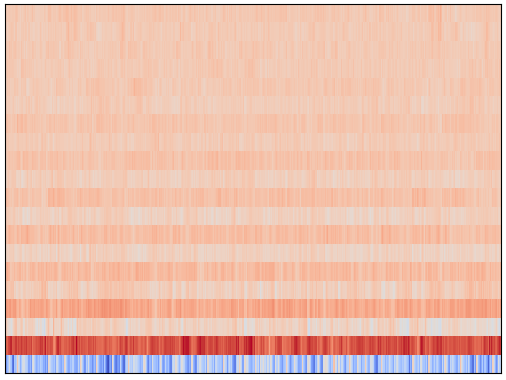
\includegraphics[width=0.9\linewidth]{mfcc.png}
\caption{Ejemplo de MFCC}
\end{figure}

Teniendo en cuenta la popularidad de los MFCC anteriormente mencionados, se puede genera un encoder. Esto asociar\'ia a cada canci\'on, a partir de su MFCC, una representaci\'on compacta de solo $500$ dimensiones; intentando guardar la mayor cantidad de informaci\'on posible de la misma. Sería muy interesante comparar el comportamiento de ambas versiones, los MFCC y el encoder reducido, para ver si se pierde informaci\'on, o se reduce el ruido al hacer esta reducci\'on de dimensiones. 

De la  m\'usica tambi\'en se puede analizar la letra, . Recientemente surgi\'o un modelo de Inteligencia Artificial de extracci\'on de letras, Whisper \cite{whisper}, lo que permite utilizar un dataset que no tenga este feature directamente. 
La letra es una caracter\'istica ligera y que intuitivamente puede aportar bastante informaci\'on sobre el g\'enero de la canci\'on. Los m\'etodos actuales de clasificaci\'on utilizando la letra utilizan técnicas de embedding de palabras como GloVe, Word2Vec\cite{classification with lyrics} y BERT \cite{bert}.  Este \'ultimo es un modelo basado en redes neuronales para el procesamiento de lenguaje natural, desarrollado por Google.

La clasificaci\'on de g\'eneros musicales basada en la Transformada de Fourier, utilizando MFCC y espectrogramas, se ha explorado extensivamente en los \'ultimos a\~nos. La Transformada de Fourier tiene una alta resoluci\'on en el dominio de la frecuencia, pero tiene una resoluci\'on cero en el dominio del tiempo. Esto significa que puede decirnos exactamente qu\'e frecuencias est\'an presentes en una se\~nal, pero no en qu\'e lugar en el tiempo se han producido \cite{wavelet transform in machine learning}.
Un mejor enfoque para analizar se\~nales con un espectro de frecuencias din\'amico es la Transformada Wavelet. Esta tiene una alta resoluci\'on tanto en el dominio de la frecuencia como en el del tiempo. Adem\'as, puede proporcionar una resoluci\'on de frecuencia variable, lo que significa que puede adaptarse a diferentes escalas de tiempo y frecuencia. 

Las caracter\'isticas mencionadas hacen de las wavelets una alternativa interesante  en la clasificaci\'on de g\'eneros musicales, donde ciertos g\'eneros pueden tener patrones r\'itmicos m\'as r\'apidos o lentos que otros \cite{Musical Genre Classification Of Audio Signals}. Por \'ultimo, ya que utiliza pocos datos para representar una se\~nal tiene gran potencial en el procesamiento de grandes cantidades de datos, como los datasets de m\'usica. 


\section{Metodología y experimentación}
Al enfrentar el problema de clasificaci\'on de g\'eneros fue realizada una investigaci\'on exhaustiva acerca de que modelos eran recomendables para cada una de las caracter\'isticas. Entre las conclusiones obtenidas resalta el hecho de que la letra, por s\'i sola no supera el 70\% de precisi\'on. Por ello fue decidido relizar una combinaci\'on innovadora entre el encoder de los MFCC y el embedding de la letra, para comprobar si la uni\'on de ambas mejora los resultados respecto a la letra sola. 

\subsection{Encoder de MFCC y embedding de la letra}
 La idea de combinar el an\'alisis de la letra y el encoder es concatenar los vectores resultantes de estos procesamientos y clasificar en base a esta combinaci\'on de features. Este modelo fue  llamado VisionLang.
 % hablar del autoencoder
 
 La arquitectura del encoder fue diseñada utilizando ideas, principalmente de \textit{An Introduction to Autoencoders} \cite{michelucci2022introduction} y \textit{Autoencoders} \cite{bank2021autoencoders}. 
 
Para construir el encoder fue programado un autoencoder y se tom\'o el modelo hasta el bottleneck. La arquitectura del autoencoder combina capas maxpooling y upsampling al inicio y al final respectivamente para moderar el tama\~no la imagen, intercaladas con capas convolucionales y en el medio, un par de capas densas para aprovechar que ya el n\'umero de dimensiones era relativamente peque\~no y realizar un poco m\'as de aprendizaje.

La arquitectura en detalle es la siguente:
\begin{table}[h!]
	\begin{center}
		\begin{tabular}{ | c | c | c |}
			\hline
			\textbf{Nombre de la capa} & \textbf{Tipo de la capa} & \textbf{Shape de salida} \\ \hline
			$input_l$ & Input & (192, 256, 3) \\ \hline
			$maxp_{ini}$ & MaxPooling2D & (96, 128, 3) \\ \hline
			$encoding_1$ & Conv2D & (96, 128, 12) \\ \hline
			$maxp_1$ & MaxPooling2D & (48, 64, 12) \\ \hline
			$encoding_2$ & Conv2D & (48, 64, 6) \\ \hline
			$maxp_2$ & MaxPooling2D & (24, 32, 6) \\ \hline
			$encoding_3$ & Conv2D & (24, 32, 3) \\ \hline
			$flat_1$ & Flatten & (2304) \\ \hline
			$bottleneck$ & Dense & (500) \\ \hline
			$decoding_1$ & Dense & (2304) \\ \hline
			$resh_1$ & Reshape & (24, 32, 3) \\ \hline
			$decoding_2$ & Conv2D & (24, 32, 6) \\ \hline
			$Up_1$ & UpSampling2D & (48, 64, 6) \\ \hline
			$decoding_3$ & Conv2D & (48, 64, 12) \\ \hline
			$Up_2$ & UpSampling2D & (96, 128, 12) \\ \hline
			$decoding_4$ & Conv2D & (96, 128, 3) \\ \hline
			$output_l$ & UpSampling2D & (192, 256, 3) \\
			\hline
		\end{tabular}
		\caption{Arquitectura del autoencoder.}
		\label{tabla:1}
	\end{center}
\end{table}

Como se puede observar la arquitectura es casi sim\'etrica.
Fue tomada como funci\'on de p\'erdida y m\'etrica el error cuadr\'atico medio ($\textit{mean squared error}$). La entrada del autoencoder y la salida esperada fueron las im\'agenes del feature MFCC del conjunto de entrenamiento luego de haber sido normalizadas, es decir, que en vez de estar en el rango $[0, 255]$ cada valor de la imagen de entrada, los representamos en el rango $[0, 1]$. 

Se probaron otras arquitecturas, desde algunas que no ten\'ian capas densas hasta otras que principalmente consist\'ian en capas densas. El problema en las arquitecturas carentes de capas densas era que sus resultados no eran lo suficientemente buenos, es decir, debido a su relativamente baja cantidad de par\'ametros el nivel de aprendizaje que pod\'ian lograr era inferior al que se logr\'o luego con arquitecturas con capas densas. Por otro lado, las arquitecturas que consist\'ian principalmente en capas densas ten\'ian problemas como que los modelos eran muy grandes, algunos pasando de los GiB de almacenamiento y presentaban un problema para nosotros a la hora del entrenamiento. Otro problema que tienen las arquitecturas m\'as basadas en capas densas es su tendencia al overfitting. En las prueba realizadas, las arquitecturas carentes de capas densas no presentaban este tipo de problema ya que los resultados en los conjuntos de entrenamiento, test y validaci\'on ten\'ian poca diferencia entre ellos, sin embargo en las arquitecturas que ten\'ian capas densas, por el gran n\'umero de par\'ametros si se evidencia una diferencia sustancial entre los resultados en los conjuntos de entrenamiento, y los obtenidos en los de prueba y validaci\'on. 


% Ahora embedding de la letra
Por cada audio del dataset se extrae la letra haciendo uso del modelo, Whisper\cite{whisper}.  Luego, se procesa la letra para obtener el embedding utilizando BERT \cite{bert}.

Una vez obtenidos los dos embedding correspondientes a la letra de la canci\'on y la m\'usica (MFCC), se conforma la capa de entrada de la red neuronal de VisionLang, o sea, la concatenaci\'on de los dos vectores obtenidos. Luego la red tiene  dos capas ocultas con funci\'on de activaci\'on RELU y cantidad de neuronas $128$ y $64$ respectivamente. Finalmente la capa de salida consiste de $10$ neuronas que representan a cada uno de los g\'eneros musicales que analizamos, y cuenta con softmax como funci\'on de activaci\'on. Siendo coherente con esto \'ultimo usamos como funci\'on de p\'erdida la Categorical Cross Entropy. Adem\'as, el modelo fue entrenado durante $500$ epochs.

\subsection{CNN-MFCC}
% ahora hablemos de MFCC y CNN
Las redes neuronales convolucionales (CNN) se utilizan ambpliamente en el campo para entrenar con MFCC, debido a que estas redes est\'an dise\~nadas espec\'ificamente para detectar patrones y caracter\'isticas en im\'agenes, lo que las hace muy \'utiles en problemas de clasificaci\'on y reconocimiento de objetos. Esto significa que no se necesita un conocimiento experto para dise\~nar los filtros o caracter\'isticas que se utilizan para procesar las im\'agenes, ya que la red es capaz de aprenderlos a partir de los datos de entrenamiento.

La arquitectura de una CNN se compone de varias capas de procesamiento, incluyendo capas de convoluci\'on y de pooling que permiten extraer caracter\'isticas relevantes de las im\'agenes de entrada. La capa de convoluci\'on es la que aplica un filtro o kernel a la imagen de entrada para detectar patrones espec\'ificos, como bordes, l\'ineas o texturas. La capa de pooling reduce la resoluci\'on de la imagen de salida, lo que ayuda a reducir el n\'umero de par\'ametros que deben entrenarse y a evitar el sobreajuste. Tambi\'en se usan capas independientemente de la necesidad del modelo, como capas para aplanar las im\'agenes a un vector, capas densas para pasarle lo que se detecto en las anteriores y ajustar pesos, y capas de activaci\'on.\\


\textbf{\large Arquitectura de capas del modelo}
\begin{itemize}
	\item Capa de entrada input: recibe la la imagen con tama\~no 256x192 y 3 filtros RGB.(256,192,3).

\item Capa Conv2D: recibe la capa input anterior y devuelve datos de tama\~no (256,192,64), aplica 64 filtros a la imagen.

\item Capa AveragePooling2D: recibe datos de tama\~no (256,192,64) y devuelve la imagen reducida en (2,2), devuelve datos de tama\~no (128,96,64).

\item Capa Conv2D: recibe datos de tama\~no (128,96,64) y devuelve datos de tama\~no (128,96,128), aplica 128 filtros a la imagen.

\item Capa AveragePooling2D recibe datos de tama\~no (128,96,128) y devuelve la imagen reducida en (2,2), devuelve datos de tama\~no (64,48,128).

\item Capa Conv2D: recibe datos de tama\~no (64,48,128) y devuelve datos de tama\~no (64,48,256), aplicando 256 filtros a la imagen.

\item Capa GlobalAveragePooling2D: recibe datos de tama\~no (128,96,128) y devuelve un vector 1D \cite{Machine Learning and Deep Learning methods for music genre Classification} de tama\~no 256, con una salida por cada filtro.

\item Capa Dense de 256 neuronas: recibe los datos de la salida de la capa anterior y los procesa con la funci\'on de activaci\'on RELU.

\item Capa Dense de 128 neuronas: recibe los datos de la salida de la capa anterior y los procesa con la funci\'on de activaci\'on RELU.

\item Capa Dense de 64 neuronas: recibe los datos de la salida de la capa anterior y los procesa con la funci\'on de activaci\'on RELU.

\item Capa Dense de 32 neuronas: recibe los datos de la salida de la capa anterior y los procesa con la funci\'on de activaci\'on RELU.

\item Capa Dense de 10 neuronas: recibe los datos de la salida de la capa anterior y los procesa con la funci\'on de activaci\'on softmax para determinar la salida de tipo clasificaci\'on.
\end{itemize}

\begin{figure}[h!] 
	\centering
	\includegraphics[width=0.9\linewidth]{CNN.png}
	\caption{CNN Model}
\end{figure}


\subsection{Audio puro con CNN 1D}
Uno de los acercamientos m\'as interesantes a la clasificaci\'on utilizando el audio puro es utilizar redes convolucionales unidimensionales (CNN 1D). La arquitectura de ResNet \cite{ResNet} es una popular red neuronal convolucional utiliza bloques residuales que permiten que la información fluya a través de la red sin perder información en el camino. Estos bloques residuales están compuestos por varias capas convolucionales y de normalización, y se utilizan para crear una red neuronal profunda con un número de capas mucho mayor que el de las redes neuronales convencionales

Cabe mencionar que, aunque el modelo est\'a inspirado en la arquitectura ResNet, la implementaci\'on en el c\'odigo no incluye las conexiones de atajo (shortcut connections) que caracterizan a ResNet. Estas conexiones permiten que las se\~nales pasen directamente a trav\'es de la red, ayudando a combatir el problema del desvanecimiento del gradiente durante el entrenamiento de redes profundas. A pesar de la ausencia de estas conexiones, el modelo a\'un puede ser efectivo para la tarea de clasificaci\'on de g\'eneros de m\'usica. Los trabajos futuros podr\'ian considerar la implementaci\'on de las conexiones de atajo para recrear m\'as fielmente la arquitectura ResNet y potencialmente mejorar el rendimiento.

La idea principal de dicho modelo es tomar una se\~nal de audio, pasarla a trav\'es de una serie de capas convolucionales para extraer caracter\'isticas \'utiles, y luego usar esas caracter\'isticas para clasificar la se\~nal en uno de los g\'eneros musicales.

La red neuronal incluye capas convolucionales, una capa de agrupaci\'on (pooling), y una capa densa (fully connected). El modelo se entrena utilizando una funci\'on de p\'erdida de entrop\'ia cruzada categ\'orica y el optimizador Adam.

\subsection{Transformada Wavelet}
La clasificaci\'on de audio utilizando la Transformada Wavelet ha ganado atenci\'on en los \'ultimos años debido a su eficacia en la captura de características locales de las se\~nales en varias escalas. Sin embargo, la investigaciones a\'un son escasas en comparaci\'on con otras t\'ecnicas de extracci\'on de caracter\'isticas. Esto puede adjudicarse a la complejidad involucrada en la selecci\'on de wavelets apropiadas y la dificultad que se le atribuye al trabajo con ellas\cite{wavelet transform in machine learning}.

\subsection {Wavelet Discretas y Complejas}
Existen tres tipos principales de wavelets: discretas, continuas y complejas. Cada tipo ofrece numerosas opciones para elegir en funci\'on de requisitos espec\'ificos, por lo que es esencial realizar investigaciones y experimentos exhaustivos antes de aplicarlos.
Debido a que las wavelets continuas se suelen analizar convertidas a im\'agenes, y a que sus resultados no son especialmente superiores a MFCC \cite{Wavelet Transform for Music Genre Classification}, la investigación fue enfocada en wavelets discretas y complejas. 

La Transformada Wavelet Discreta (DWT) \cite{wavelet transform in machine learning} es un caso especial de Transformada Wavelet que proporciona una representaci\'on compacta de la se\~nal en el tiempo y la frecuencia, que se puede calcular de manera eficiente\cite{Musical Genre Classification Of Audio Signals}. Por otro lado  la Transformada Wavelet Compleja de Doble \'arbol (DT-CWT) \cite{DT-CWT} es una mejora relativamente reciente a DWT; ya que para se\~nales moduladas complejas como el audio, DWT encuentra algunas pocas deficiencias: oscilaciones, varianza de desplazamiento, aliasing y falta de direccionalidad \cite{Wavelet Transform for Music Genre Classification}.

Respecto a la Transformada Wavelet Discreta, Daubechies wavelet  emp\'iricamente muestra el mejor comportamiento en muchas aplicaciones\cite{Wavelet Transform for Music Genre Classification}. En las pruebas con distintos \'ordenes de Daubechies wavelet, db12 fue la que mejor se desempe\~n\'o. Por otro lado la Transformada Wavelet Compleja de Doble \'arbol, mostr\'o los mejores resultados con 17 niveles de descomposici\'on.

Teniendo en cuenta las recomendaciones de \cite{wavelet transform in machine learning}, varios de los modelos de machine learning tradicional son muy prometedores en aprendizaje con wavelets. Para la experimentaci\'on preliminar fue analizado el comportamiento de dichos modelos en GTZAN (como se puede ver en la tabla), destac\'andose Random Forest Classifier y Gradient Boosting Classifier.

\begin{table}[htbp]
\centering
\begin{tabular}{|l||c|c|}
\hline Modelo \ Feature & DWT & DT-CWT\\ %
\hline\hline Random Forest & 0.7487 & 0.7527 \\ 
\hline Gradient Boosting & 0.7497 & 0.7467 \\ %
\hline Logistic Regression & 0.6857 & 0.7297 \\ %
\hline Linear SVC & .6637 & 0.7227 \\ 
\hline SVC & 0.6486 & 0.6847 \\ %
\hline
\end{tabular}%
\caption{Precisión promedio en 5-Fold} 
\label{tabla:2}%
\end{table}

\section{Resultados}
El dataset fue dividido en 80\% para entrenar, 10\% para validar y 10\% para pruebas, manteniendo el balance de cantidad de elementos por cada clase, para todos los conjuntos.

El modelo de CNN utilizando MFCC, tras 300 \'epocas de entrenamiento, mostr\'o una precisi\'on de 0.7879 en los datos de prueba, 0.7699 en los de validaci\'on y 0.9786 en los de entrenamiento.

Se muestran en los siguientes gr\'aficos los resultados del entrenamiento en el transcurso de las \'epocas. Se puede apreciar que cuando los datos de entrenamiento pierden el sobreajuste, los datos de validaci\'on por lo general mejoran el resultado. En esos picos se nota c\'omo el modelo generaliza mejor.

\begin{figure}[h!] 
	\centering
	\includegraphics[width=0.9\linewidth]{CNN_accuracy.png}
	\caption{CNN Accuracy}
\end{figure}

\begin{figure}[h!] 
	\centering
	\includegraphics[width=0.9\linewidth]{CNN_loss.png}
	\caption{CNN Loss}
\end{figure}

Tambi\'en se reporta una matriz de confusi\'on para comprobar
el comportamiento en cada g\'enero. Se observa que no
se desempe\~na de la misma forma en todos los g\'eneros,
ya que hay algunos (como el country) donde se
observan mejores resultados que en otros (reggae).

\begin{figure}[h!] 
	\centering
	\includegraphics[width=0.9\linewidth]{CNN_confusion.png}
	\caption{Matriz de confusi\'on}
\end{figure}

En la siguiente tabla se muestran los resultados de test por cada g\'enero:
\begin{table}[h]
\centering
\begin{tabular}{|c|c|}
\hline
\textbf{Genre} & \textbf{Accuracy} \\ \hline
blues & 0.551 \\ \hline
classic & 0.851 \\ \hline
country & 1.000 \\ \hline
disco & 0.852 \\ \hline
hip hop & 0.749 \\ \hline
jazz & 0.827 \\ \hline
metal & 0.949 \\ \hline
pop & 0.651 \\ \hline
reggae & 0.759 \\ \hline
rock & 0.551 \\ \hline
\textbf{average} & \textbf{0.787} \\ \hline
\end{tabular}
\caption{Precisi\'on de clasificaci\'on por cada g\'enero de GTZAN.}
\label{tabla:3}
\end{table}

Al entrenar el autoencoder se realiz\'o un $save$ cada $10$ epochs. En la siguiente imagen se observan los resultados sobre el n\'umero del $save$ en el modelo de autoencoder presentado:
\begin{figure}[h!]
	\centering
		\includegraphics[width=0.9\linewidth]{overfitting_graph.png}
		\caption{Gr\'afica de error del modelo contra n\'umero de \'epocas del entrenamiento.}
\end{figure}

A partir del an\'alisis de la gr\'afica anterior se tom\'o como cantidad de epochs a ejecutar la cantidad de $150$, ya que se conjetur\'o (y luego valid\'o) que el comportamiento del modelo en el conjunto de prueba ser\'ia muy similar al comportamiento en el conjunto de validaci\'on y en este punto es que se obtiene un mejor performance en el conjunto de prueba. 

Volviendo atr\'as, los resultados obtenidos para cada tipo de modelo:
\begin{itemize}
	\item los modelos que no ten\'ian capas densas lograron primeramente un error (MSE) de $0.0025$ y luego de ampliar la   cantidad de dimensiones que salen del bottleneck, es decir la cantidad de dimensiones de la representaci\'on se logr\'o $0.0021$. Estos modelos ten\'ian muy poco overfitting luego de $500$ epochs.
	\item los modelos que presentan capas densas, por su parte, comenzaron con resultados en el conjunto de entrenamiento de hasta $0.0011$ con $500$ epochs, lo cual era muy bueno pero pod\'ia implicar overfitting. A medida que se redujeron la cantidad de par\'ametros (de $288$ millones a los $2.3$ millones del modelo propuesto) los resultados en el conjunto de entrenamiento fueron peores pero nunca sobrepasaron el valor de $0.0013$ en $500$ epochs. Luego de correr el modelo propuesto solo $150$ epochs se obtuvieron los mejores resultados tanto en el conjunto de prueba como en el validaci\'on, oscilando alrededor de $0.00185$, por su lado en el conjunto de entrenamiento se obtuvieron resultados alrededor de $0.0016$, lo que evidencia la presencia de overfitting.
\end{itemize}

Se realiz\'o tambi\'en cross validation con Kfold dividiendo todo el conjunto de entrenamiento en $10$ subconjuntos. Los resultados del cross validation coincidieron con los resultados anteriormente descritos. Este test se hizo luego de haber fijado la cantidad de epochs en $150$.

VisionLang, que fue entrenado durante $500$ epochs, presenta una precisi\'on, para el conjunto de entrenamiento, casi perfecta llegados al epoch n\'umero $300$. En el caso del conjunto de  datos de validaci\'on, que es el que nos da la efectividad de nuestro modelo, vemos que el accuracy crece r\'apidamente hasta llegar al valor $0.57$ alrededor del epoch $150$. 

\begin{figure}[h!]
	\centering
	\includegraphics[width=0.9\linewidth]{vl_accuracy.png}
	\caption{Gr\'afico de precisi\'on}
\end{figure}

Con m\'as capas y neuronas el modelo hac\'ia r\'apidamente overfitting, o sea en pocos epochs. Esto nos llev\'o a reducirlo a la arquitectura actual. Como podemos observar en la pr\'oxima gr\'afica la funci\'on de p\'erdida para los datos entrenantes decrece r\'apidamente acerc\'andose mucho a cero en el epoch $300$. En el caso de los datos de validaci\'on, vemos como a partir del epoch $100$ la red comienza a hacer overfitting, pero no es representativo. 

\begin{figure}[h!]
	\centering
	\includegraphics[width=0.9\linewidth]{vl_loss.png}
	\caption{Gr\'afico de funci\'on de p\'erdida}
\end{figure}

Presentamos aqu\'i adem\'as la matriz de confusi\'on.

\begin{figure}[h!]
	
	\centering
	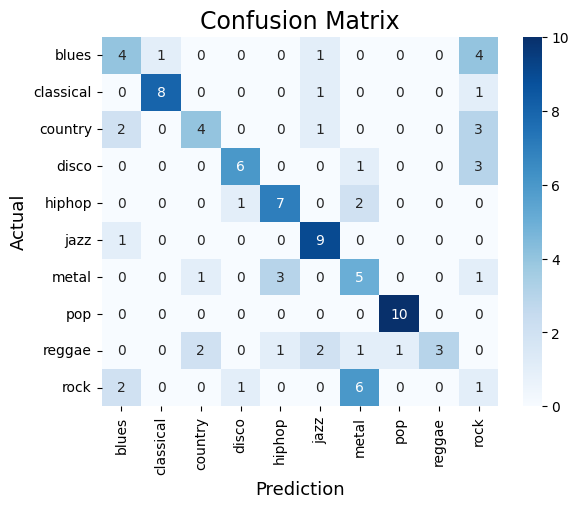
\includegraphics[width=0.9\linewidth]{vl_confussion_matrix.png}
	\caption{Matriz de Confusi\'on}
\end{figure}

Finalmente con un accuracy de $0.57$ y con valor para la funci\'on de p\'erdida de  $2.9323$ llegamos a la conclusi\'on de que este modelo no arroja resultados que mejoren los obtenidos en los modelos ya vistos anteriormente.

En la experimentaci\'on con wavelets, despu\'es de un an\'alisi m\'as exhaustivo, se pudo deducir que los mejores resultados provienen del uso de DT-CWT con Random Forest, que al probarlo en el 20\% de GTZAN muestra 78\% de precisi\'on.

\begin{figure}[h!] 
\centering
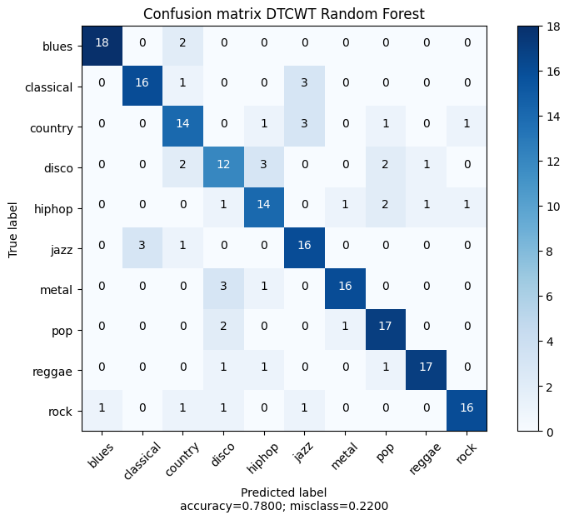
\includegraphics[width=0.9\linewidth]{ConfM_DTCWT_rf.png}
\caption{Matriz de confusi\'on de Random Forest con DT-CWT}
\end{figure}

Para corroborar los resultados anteriores fueron realizadas 30 iteraciones de Cross Validation donde la precisi\'on promedio fue de 0.7797, y la desviaci\'on est\'andar de 0.0819. Sin embargo hubo muchas instancias con valores superiores a 0.90, la mayor alcanzando 0.97 de precisi\'on. 

\begin{figure}[h!] 
\centering
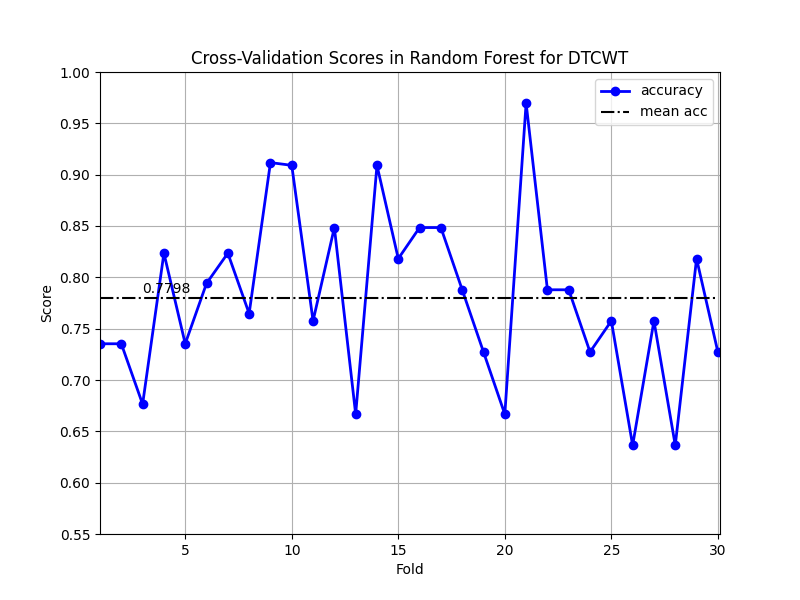
\includegraphics[width=0.9\linewidth]{CV_DTCWT_rf.png}
\caption{DT-CWT Cross-Validation}
\end{figure}

\section{Ensemble}

Como modelo final del proyecto se propuso crear un ensemble para mezclar resultados de distintos modelos preentrenados por separado y asi aprovechar la fortaleza de cada uno de estos. Se decidio usar el tipo de ensemble staking. Este consiste en entrenar los modelos base y el modelo final(el ensemble) con conjuntos de datos distintos. Para el entrenamiento se dividi\'o la base de datos en 56\% para entrenar los modelos base, 12\% para validar, 12\% para probar(test) y 20\% para entrenar el modelo final.

\textbf{\large Arquitectura}\\
La arquitectura de este modelo es simple, es un modelo secuencial que consta de una capa densa de entrada con 100 neuronas con funci\'on de activacion relu, a la cual se le pasa el resultado de las predicciones de los modelos preentrenados, ergo la capa tendr\'a como entrada una lista de vectores, donde la posici\'on $i$ del vector indica el resultado predicho por el $i$-\'esimo modelo que que pertenece a los modelos que se utilicen en una iteraci\'on dada(los modelos a usar en el ensemble son maleables).
Seguido de esta capa le siguen dos capas densas m\'as ambas de 100 neuronas y activacion relu, cierra con una capa densa de 10 neuronas con funcion de activacion softmax y con ello la salida del modelo sera un numero entre [0,9], el cual representara un genero dado.

\begin{figure}[h!] % Start the main figure environment
	\centering
	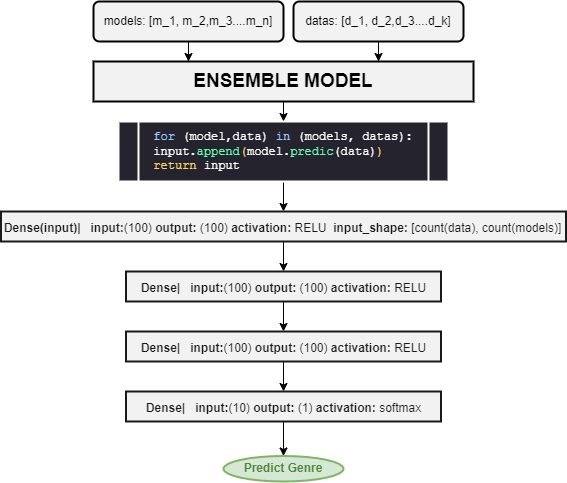
\includegraphics[width=0.9\linewidth]{ensemble.png}
	\caption{Modelo del ensemble}
\end{figure}
\textbf{\large Resultados}\\
Dado que la base de datos utilizada contiene una cantidad relativamente peque\~na de datos al entrenar los modelos base con solo un 56\% de los datos se obtuvieron los resultados: 

\begin{itemize}
\item mfcc-cnn: 0.61 test accuracy
\item wavelets: 0.60 test accuracy 
\end{itemize}

Al entrenar el modelo final con el 20\% de los datos restantes se obtuvo una precisi\'on de 0.65, lo cual si bien no es mejor resultado que los modelos entrenados individualmente con un conjunto de datos m\'as amplio, es un resultado que nos indica que en trabajos futuros con datasets m\'as abarcadoras, o con una dataset ampliada que tenga suficientes datos para preentrenar bien los modelos base, el ensemble mejora los resultados de los modelos previamente entrenados aprendiendo de las fortalezas de cada uno de estos.


	\section{Recomendaciones}
  
Un aspecto cr\'itico que afecta el rendimiento de los modelos de clasificaci\'on radica en la precisi\'on y consistencia de las anotaciones asignadas manualmente. Los esfuerzos futuros deber\'ian priorizar la recopilaci\'on de datos de mayor calidad a trav\'es de pautas m\'as estrictas, anotaciones de expertos o procedimientos de ratificaci\'on de colaboraci\'on colectiva.

Otro enfoque para impulsar el rendimiento de los modelos de clasificaci\'on de g\'enero es combinar m\'ultiples modelos a trav\'es de ensembles. Al integrar predicciones de distintos algoritmos y representaciones de caracter\'isticas, los ensembles aprovechan las fortalezas de los clasificadores individuales mientras mitigan sus debilidades.  

  Al seguir estas direcciones, los investigadores pueden ampliar nuestra comprensi\'on de la clasificaci\'on de g\'eneros musicales y sentar bases s\'olidas para soluciones de pr\'oxima generaci\'on en \'areas relacionadas, incluido el an\'alisis de audio, la recuperaci\'on de informaci\'on o las interfaces interactivas centradas en el ser humano.
  
	    
	\begin{thebibliography}{20}
		\bibitem{whisper} A. Radford, J. Wook Kim, T. Xu, G. Brockman, C. McLeavey y I. Sutskever: \emph{Robust Speech Recognition via Large-Scale Weak Supervision}. Preprint on arXiv: 2212.04356, 2022. 	
		\bibitem{Conv1D} Safaa Allamy, Alessandro Lameiras Koerich: \emph{1D CNN Architectures for Music Genre Classification}. Preprint on arXiv.2105.07302, 2021. 
		\bibitem{ResNet} Kaiming He, Xiangyu Zhang, Shaoqing Ren, Jian Sun: Deep Residual Learning for Image Recognition, 2015
		\bibitem{bert} J. Devlin, M. Chang, K. Lee y K. Toutanova: \emph{BERT: Pre-training of Deep Bidirectional Transformers for Language Understanding}. Preprint on arXiv: 1810.04805, 2018. 
		\bibitem{classification with lyrics} Megan Leszczynski, Anna Boonyanit: \emph{Music Genre Classification using Song Lyrics}, 2021.
		\bibitem{murphy} Kevin P. Murphy: \emph{Machine Learning: A Probabilistic Perspective}. MIT Press, 2012.
		\bibitem{Wavelet Transform for Music Genre Classification} Pranav Vijaya Kumar Rao, Vishwas Nagesh Moolimani: \emph{ECG Analysis based feature extraction using Wavelet Transform for Music Genre Classification}, 2020. 
		\bibitem{wavelet transform in machine learning} Ahmet Taspinar: \emph{A guide for using the wavelet transform in machine learning}, unpublished. [Online]. Available: http://ataspinar.com/2018/12/21/a-guide-for-using-the-wavelet-transform-in-machine-learning/
		\bibitem{DT-CWT} Selesnick, I.W. and Baraniuk, R.G. and Kingsbury, N.C., \emph{The dual-tree complex wavelet transform}, 2005, IEEE Signal Processing Magazine, pp. 123-151.
		\bibitem{Wavelets y sus Aplicaciones} Liliana R. Castro, Silvia M.  Castro: \emph{Wavelets y sus Aplicaciones}, ler. Congreso Argentino de Ciencias de la Computaci\'on, pp. 195-204.
		\bibitem{Musical Genre Classification Of Audio Signals} George Tzanetakis, Georg Essl, Perry Cook: \emph{Automatic Musical Genre Classification Of Audio Signals}
		\bibitem{Machine Learning and Deep Learning methods for music genre Classification} Rusian Gohkman: \emph{Machine Learning and Deep Learning methods for music genre Classification}
		\bibitem{mfcc wikipedia} Mel-frequency cepstrum (s.f.). Wikipedia.  [Online]. \url{https://en.m.wikipedia.org/wiki/Mel-frequency_cepstrum}, junio 2023.
		\bibitem{michelucci2022introduction} Umberto Michelucci: \emph{An Introduction to Autoencoders}. Preprint on arXiv: 2201.03898, 2022.
		\bibitem{bank2021autoencoders} Dor Bank and Noam Koenigstein and Raja Giryes: \emph{Autoencoders}. Preprint on arXiv: 2003.05991, 2021.
    \end{thebibliography}
	
\end{document}
